\chapter{Appendix: how to assemble the drone}\label{app:build}
This chapter describes how to build and assemble all the components for both drone models presented in Chapter \ref{ch:hw} and it is useful for readers that do not find the present hardware design intuitive or that are not familiar with these DIY projects.

\section*{Board and sensors}

\begin{enumerate}
    \item On the PCB bottom side, soldier sets of female pins for the ADC module and the GPIO0. 
    On the top side, soldier the resistances and sets of male pins for the ESCs, telemetry and GPS-compass; soldier sets of female pins for the receiver, UART-USB adapter, the barometer and IMU.
    
    
    For the battery feedback and power supply pins (for the FPGA, and the +5v coming from the power module in Model-B units) the ground pins are male and voltage input are female.
    
\begin{figure} [H]
    \centering
    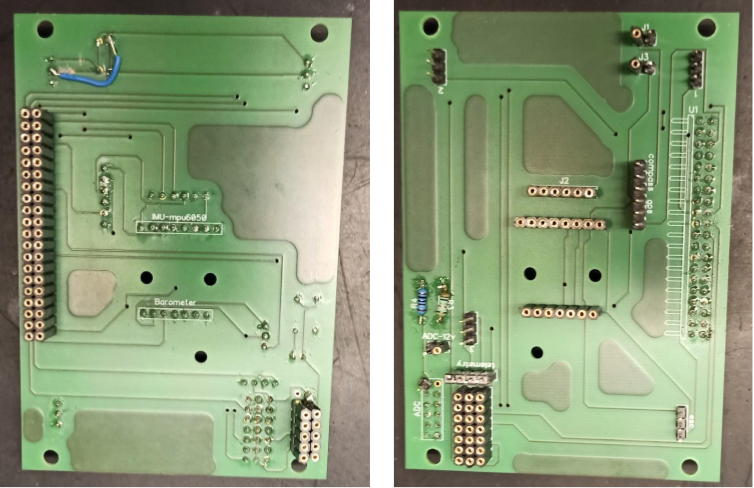
\includegraphics[scale=0.5]{Figures/build/PCB_topBottom.png}
    \caption{Pins soldier to the PCB on the bottom side (left) and top (right).}
    \label{fig:build_pins}
\end{figure}
    
    \item To attach the PCB to the FPGA, it is necessary to make the female pins on the bottom side longer, so add a second round of female pins on top of the soldiered ones. Once the PCB can be placed on top of the FPGA, use screws M3 on the corners to attach it.
    
    
    \item Add the IMU, barometer, UART-USB adapter and receiver to the top side of the PCB. Watch out for the height of the sensors.
    
    
    \item Attach the steppers to the central holes of the FPGA-Frame attachment. Afterwards, attach the part to the bottom of the FPGA.
    
\end{enumerate}


\begin{figure} [H]
    \centering
    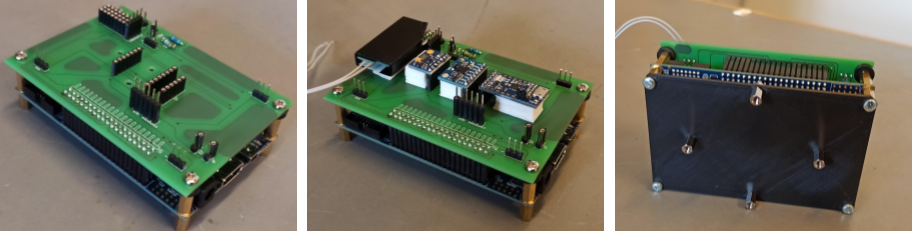
\includegraphics[width=\textwidth]{Figures/build/PCB_FPGA.png}
    \caption{Board building steps nr.2 (left), 3 (center) and 4 (right).}
    \label{fig:build_board}
\end{figure}

\section*{Main body assembly}

\begin{enumerate}
    \item Soldier the ESCs power supply and battery X66 connector to the bottom part of the frame.
    
    \item Soldier as well two additional wires for the battery feedback on the top-right ESC. It is not mandatory that the wires are blue, but this color was chosen for this project since it makes it easier to differentiate from the other components.
    
    \item Screw the arms and legs to the bottom part of the frame. Also attach with a zip or tape the ESCs to the arms. As a convenience, the two red arms are meant for the front side and the two white for the back.
    
    \item Turn the body upside down and screw the top part of the frame (except for the screws that are for the cover).
    
\begin{figure} [H]
    \centering
    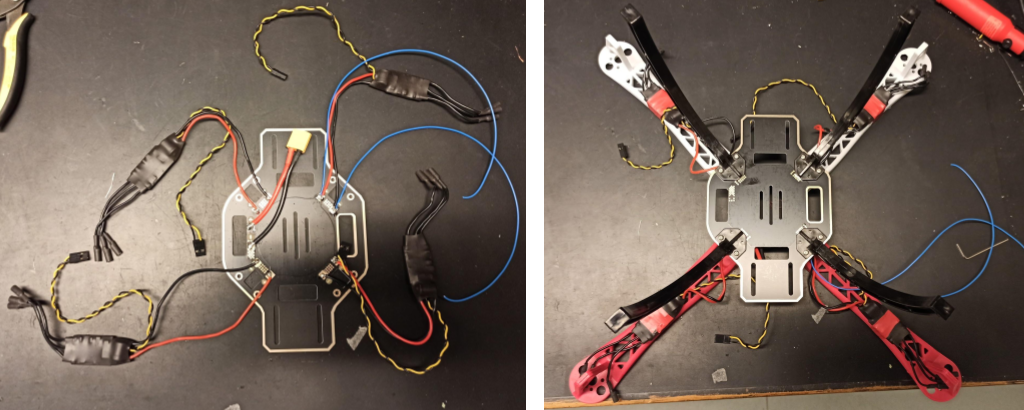
\includegraphics[width=\textwidth]{Figures/build/frame_123.png}
    \caption{Frame building steps nr.1 and 2 (left), 3 and 4 (right).}
    \label{fig:build_frame1234}
\end{figure}
    
    \item Screw the motors on the arms and connect them to the ESCs. DO NOT zip/tape these connectors yet.
    
    \item Add a belt for the battery on the bottom. In case of building a Model-B unit, also connect the power module to the battery connector of the bottom.
    
    \item Attach the telemetry module to the top. Watch out for the screws on the top and avoid covering the holes for the FPGA and cover.
    
\begin{figure} [H]
    \centering
    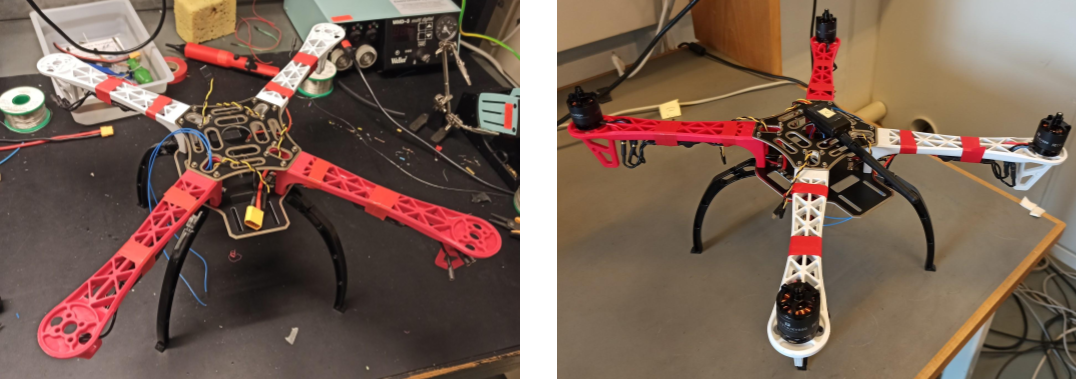
\includegraphics[width=\textwidth]{Figures/build/frame_45.png}
    \caption{Frame building steps nr.5 and 6 (left), 7 (right).}
    \label{fig:build_frame567}
\end{figure}

    \item Attach the FPGA+PCB from the previous section with the steppers. Notice that the IMU's X axis must point to the front. For a more visual understanding, the receiver placement must be between the two red arms.
    
    \item Connect the ESCs, telemetry and battery feedback to the board.
    
    \item To download a C-App without removing the cover, add a USB connector (male USB-B mini - female USB) that goes from the UART-USB adapter to the outside of the frame (just down the bottom part, see Figure \ref{fig:hw_space}).
    
    \item Add the drone number to the cover and attach the GPS to its cavity using the CGPS-Cover attachment. It is not mandatory that the drone number is the same as the telemetry pair number, but this makes it easier for working with multiple drones.
    
\begin{figure} [H]
    \centering
    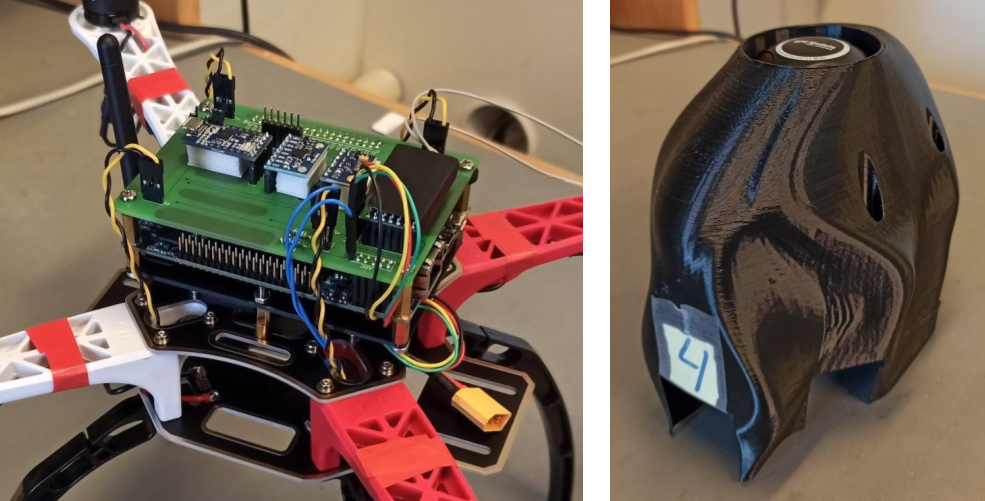
\includegraphics[width=\textwidth]{Figures/build/frame_board.png}
    \caption{Frame complete wiring (left) and finished cover (right).}
    \label{fig:build_frameBoard}
\end{figure}
    
    \item Connect the GPS to the PCB and screw the cover to the frame.
    
    \item In case of using a brand new set of motors, run the ESC calibration program to enable the motors and make them work properly.
    
    \item Run the test program for the motors and verify that the four motors spin in the correct direction. In case a motor spins in the wrong direction, switch two of its connections with the ESC.
    
\end{enumerate}

\textbf{\textit{NOTE:}} Before attaching the cover to the frame, check that the devices and the board are functional. Download Patmos and run the test programs for all the devices to verify the components are functional. Check the Appendix \ref{app:setup} to see how to do so.

In case of some devices, it is necessary to modify their settings when they are brand new (or used for the first time) in order to be compatible work with Patmos and the flight controller, see the Section \ref{app:sec_fc}.

% ===================================================================================
% Add this chapter to the table of contents:
%\addcontentsline{toc}{chapter}{Appendix: how to assemble the drone}